\documentclass{report}
\usepackage[utf8x]{inputenc}
\usepackage[T1]{fontenc}
\usepackage[francais]{babel}
\usepackage{graphicx}
\usepackage{hyperref}
\usepackage{verbatim}

\addtolength{\oddsidemargin}{-.575in}
\addtolength{\evensidemargin}{-.575in}
\addtolength{\textwidth}{1.75in}
\addtolength{\topmargin}{-.875in}
\addtolength{\textheight}{1.75in}


\author{Léo Unbekandt - Guillaume Paran - Lucas Saurel}
\date{Mai 2012}
\title{Projet web - UnsapaIPW}
\begin{document}

  \maketitle
  \clearpage
  \tableofcontents
  \clearpage

  \section*{Introduction}
  \addcontentsline{toc}{chapter}{Introduction}
    Le $2^e$ sujet nous a été attribué. Il s'agissait de réaliser une plateforme
    de gestion d'examens sur laquelle des professeurs peuvent créer des examens
    et les étudiants doivent alors déposer un fichier qui soit accessible pour
    le professeur en guise de rendu. Le sujet nous imposait un certain nombre de
    cas d'utilisation auxquels nous avons répondu.

    Un des points importants de l'application étaient la gestion des droits.
    Selon chaque rôle, les utilisateurs ne doivent pas voir la même chose
    pour une ressource donnée. Par exemple, pour les examens : un étudiant doit voir
    ceux auxquels il est inscrit tandis qu'un professeur doit voir ceux dont il est 
    responsable.

  \clearpage
    
  \chapter{Fonctionnalités de l'application}
    \section{Gestion des rôles}
      L'application web que nous avons réalisée est un système de gestion 
      d'examens. On distingue trois catégories d'utilisateurs:

      \begin{itemize}
        \item{Les étudiants : ils consultent les examens auxquels leur promotion 
          est inscrite et déposent leurs compositions.}
        \item{Les responsables d'examens : ils créent des examens et notent les 
          étudiants.}
        \item{L'administrateur : il gère l'ensemble des utilisateurs, des 
          promotions et des examens.}
      \end{itemize}

    \section{Les différentes \textsl{user stories}}
       \subsection{Un utilisateur s'inscrit}
        Lorsqu’un utilisateur s’inscrit son compte est immédiatement activé, mais
        nous pouvons configurer notre application pour qu’un mail soit envoyé avec une
        URL de validation (Chemin : app/config/config.yml).
        \begin{verbatim}
          Route : /register 
          Controller : FOSUserBundle:RegistrationController
        \end{verbatim}

      \subsection{Un utilisateur s'authentifie}
        Si l'utilisateur ne clique pas directement sur \textsl{se connecter}, il lui sera demandé
        de s'authentifier lorsqu'il tentera d'accéder à des pages où un utilisateur inconnu
        n'a pas le droit d'accès. Les mots de passe sont stockés en sha1 dans la base de données,
        personne à part leur propriétaire ne peut les récupérer.
        \begin{verbatim}
          Route : /login 
          Controller : FOSUserBundle:SecurityController
        \end{verbatim}

      \subsection{Un respo TD crée un examen}
        Si un utilisateur a le rôle de responsable de TD, il a la possibilité
        de créer des examens.        
        \begin{verbatim}
          Route : /exams/add
          Controller : ExamsController
          Action : addAction
        \end{verbatim}

      \subsection{Un respo TD gère les étudiants associés à un examen}
          Lors de l'ajout d'un examen, le respo TD choisit une promotion. Par défaut
          tous les étudiants de cette promotion seront associés. Cependant, il peut
          s'il le souhaite cliquer sur détails et sélectionner 
          précisément les participants à l'examen.
          Sur la page listant les examens dont il est responsable, il peut
          cliquer sur "Gérer les étudiants" et accéder à une page où,
          de la même manière, il pourra gérer plus finement les
          étudiants qui sont concernés:
              \vspace{1em}
              \begin{verbatim}
                Route : /exams/{:examid}/students
                Controller : AttendController
                Action : examChoiceAction
              \end{verbatim}

     \subsection{Un étudiant consulte la liste des examens auxquels il est associé}
        \begin{verbatim}
          Route : /exams 
          Controller : ExamsController
          Action : indexAction
        \end{verbatim}

      \subsection{Un étudiant dépose un rendu}
        Un étudiant peut proposer un rendu pour chaque examen auquel il a été inscrit.
        Lorsqu'il choisit l'examen pour lequel rendre un document, il est averti s'il a
        déjà rendu quelque chose. L'interface lui propose également de télécharger l'ancienne
        version de son travail.
        Les fichiers DOC, DOCX, PDF et ZIP sont acceptés. Nous faisons
        la vérification par rapport aux mime-types et pas seulement par rapport aux extensions.
        Page de soumission :
        \begin{verbatim}
          Route : /register/submit
          Controller : ExamsController
          Action : submitAction
        \end{verbatim}
        Téléchargement de fichier :
        \begin{verbatim}
          Route : /download/{:examid}/{:userid}
          Controller : AttendController
          Action : downloadAction
        \end{verbatim}

      \subsection{Un respo TD attribue une note à un document déposé}
        Lorsqu'un examen est terminé, le responsable peut commencer à noter les rendus.
        Il ne peut pas le faire avant car nous laissons aux étudiants la possibilité
        de modifier leur rendu jusqu'au dernier jour.
        Sur la page qui liste les examens dont il est responsable
        (/exams), dans la partie "Examens terminés",
        un responsable a accès à la liste des étudiants. Il voit ceux qui
        n'ont rien rendu, et ceux qui ont proposé un document. Il peut alors
        télécharger ce qui a été proposé et noter.
        (/download/{:examid}/{:userid})
        Afin de faciliter l'ordre sur l'ordinateur du responsable, les documents
        téléchargés ont un nom sous la form "nomexamen\_nométudiant.ext".
        \begin{verbatim}
          Route : /exams/{:examid}/marks
          Controller : AttendController
          Action : markStudentsAction
        \end{verbatim}

      \subsection{Un utilisateur consulte les moyennes par promo}
        Une page avec des statistiques simples est proposée pour tous les utilisateurs,
        même les non-identifiés.
        \begin{verbatim}
          Route : /stats
          Controller : StatsController
          Action : indexAction
        \end{verbatim}

      \subsection{Un administrateur gère les promos}
        Il existe un utilisateur ayant le rôle d'administrateur sur le site. Il
        a accès à un panneau d'administration d'où il va pouvoir 
        ajouter/modifier/supprimer des promotions, voir/modifier/(dés)activer/changer de rôle
        les comptes utilisateurs.
        \begin{verbatim}
          Route : /admin
          Controller : AdminController
          Action : indexAction
        \end{verbatim}
 
    \section{Ce que nous n'avons pas fait}
    \subsection{Génération des mots de passe}
        Il est demandé dans le sujet de générer aléatoirement un mot de passe lors 
        de l'inscription d'un nouvel utilisateur. Nous utilisons un Bundle qui 
        gère toute la partie identification, enregistrement, récupération de mots
        de passe, gestion du profil… Ainsi pour redéfinir la manière dont l'enregistrement
        est géré, il était nécessaire de redéfinir un certain nombre de classes
        (concrètement le controller, le formtype, le handler et le template). Nous
        avons considéré que c'était beaucoup de temps de travail pour une petite fonctionnalité
        et nous sommes donc plutot concentrés sur des tâches plus prioritaires.
        
        
      \subsection{3 états pour les examens}
        Le sujet demandait à ce qu'un examen puisse être :

        \begin{itemize}
          \item{En création}
          \item{En cours}
          \item{Clos}
        \end{itemize}

        Dans notre application, nous nous basons sur la date d'échéance de l'examen
        En l'occurrence, un examen dont la date n'est pas encore passée est "en cours"
        tandis qu'un examen dont la date est passée est "clos" et la notation peut commencer.
  	
  \chapter{Schéma de données}
    Le sujet nous imposait d'utiliser plusieurs entitées auxquelles nous avons 
    ajouté un certain nombre d'attributs.

    Voici le schéma relationnel de notre base de données, avec les relations entre les 
    différents modèles :
    \begin{figure}[!h]
      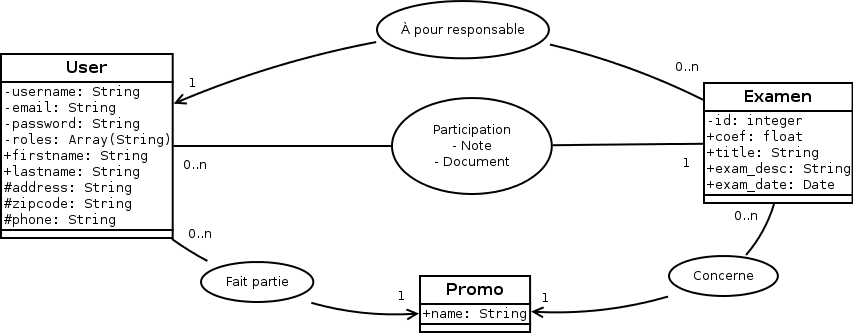
\includegraphics[width=0.9\textwidth]{./data.png}
      \caption{Schéma relationnel}
    \end{figure}

    En découle la modélisation exacte de nos données telles qu'elles sont stockées en base :
    \begin{figure}[!h]
      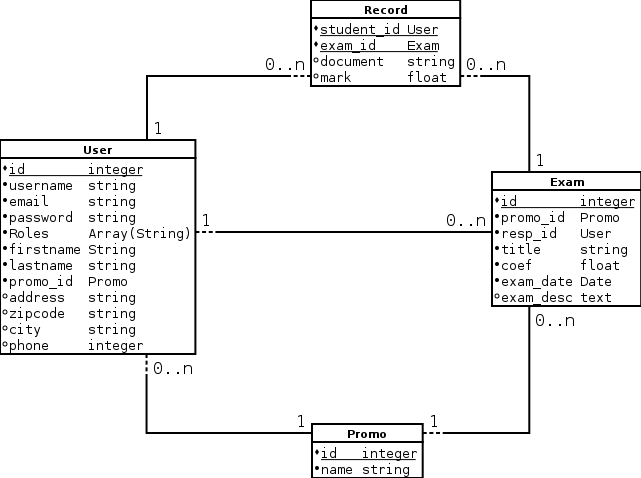
\includegraphics[width=0.9\textwidth]{./db.png}
      \caption{Modèle physique de base de données}
    \end{figure}
    \clearpage

    \section{User}
      En plus des champs prérequis :
      \begin{itemize}
        \item{Prénom}
        \item{Nom}
        \item{Adresse}
        \item{Code postal}
        \item{Ville}
        \item{Adresse e-mail}
        \item{Numéro de téléphone}
      \end{itemize}\vspace{1em}

      Le UserBundle nous rajoute toute la partie nécessaire à la gestion de
      l'utilisateur côté serveur.
      \begin{itemize}
        \item{Le mot de passe $\Rightarrow$ chiffré en sha1 dans la BDD}
        \item{Les rôles $\Rightarrow$ Pour la gestion des permissions}
        \item{Nom d'utilisateur}
        \item{Expiration du compte, confirmation par email etc.}
      \end{itemize}\vspace{1em}

      Enfin, nous avons ajouté un champ promotion. En effet, on considère 
      qu'un étudiant appartient à une promotion précise.

    \section{Promo}
      Les promotions correspondent à un regroupement d'utilisateurs, dans le cas
      d'utilisation présent, tous les étudiants d'une même année appartiennent 
      à une promotion unique.


    \section{Exam}
      Un examen représente une épreuve définie par un enseignant. L'examen 
			comprend les propriétés suivantes :
			\begin{itemize}
				\item{Titre}
				\item{Descrption}
				\item{Promotion}
				\item{Coefficient}
				\item{Date limite}
				\item{Responsable : Un user responsable de TD}
      \end{itemize}\vspace{1em}

			Par défaut, lors de la création de l'examen, tous les étudiants de la 
      promotion sélectionnée sont concernés par l'examen, mais il est également 
      possible de modifier au cas par cas si un étudiant est affecté par l'examen.
      
    \section{Record}
			L'entité Record fait le lien entre les étudiants et les examens. En effet
      dans un record on attribue pour un étudiant et un examen, la note, ainsi
      que le document rendu (Fichier pdf ou word).

			On a donc :
			\begin{itemize}
				\item{Étudiant}
				\item{Examen}
				\item{Note}
				\item{Document}
      \end{itemize}\vspace{1em}

			Ainsi un Record avec la note et le document NULL, correspond au fait qu'un
      étudiant doit effectuer un rendu pour un tel examen. Quand il rend quelque
      chose, on peuple le champ 'Document'. Quand la date de rendu est passée,
      le responsable de l'examen peut associer une note.

  \clearpage
  \chapter{Réalisation Technique}
    \section{Symfony2}
      Contrairement à ce qui a été vu en cours, nous avons choisi d'utiliser la 
      version 2 du framework symfony. Pourquoi avons nous fait ce choix ? Nous 
      trouvions intéressant de nous porter sur une technologie plus neuve que 
      Symfony 1.x, en pensant que d'ici quelques années, cette version sera bien
      plus utilisée dans des projets qu'une plus ancienne version.
      
      En outre, cela nous a permis d'accumuler d'un côté les connaissances sur
      Symfony 1.x du cours, et en plus ce qui a été fait dans Symfony2. D'un point de vu 
      pédagogique, nous avons bien plus appris de cette manière.
      
      De plus la communauté Symfony s'est massivement adaptée à Symfony2, ainsi
      de nombreux plugins sont aujourd'hui disponibles, grâce au projet \textsl{Composer}
      \footnote{\href{http://getcomposer.org/}{http://getcomposer.org/}}
      , un gestionnaire de paquets pour PHP très utilisé dans cet écosystème,
      à la manière des gems en Ruby\footnote{\href{https://rubygems.org/}{https://rubygems.org/}}
.
      

    \section{UserBundle}
      Nous avons utilisé un Bundle d'extension nommé : 
      \href{https://github.com/FriendsOfSymfony/FOSUserBundle}{UserBundle}.
      
      Ce bundle constitue la brique applicative qui permet d'ajouter un grand
      nombre de fonctionnalités nécessaires à la plupart des projets :
      \begin{itemize}
        \item{Inscription}
        \item{Authentification}
        \item{Connexion}
        \item{Déconnexion}
        \item{Gestion du profil}
        \item{Changement de mot de passe}
      \end{itemize}\vspace{1em}

      L'utilisation de ce Bundle nous a permis d'éviter un travail long
      et inutile sur le plan métier de l'application.
      
    \section{Jeu de données}
        Afin de pouvoir effectuer des tests, nous avons mis en place un jeu de
        données comprenant plusieurs utilisateurs. Les mots de passe utilisés
        sont identiques aux noms d'utilisateur.
        Pour s'authentifier en tant qu'administrateur il suffit d'utiliser
        l'identifiant 'admin'.
        Les différents responsables de TD capables de gérer les examens et de
        noter les étudiants sont :
        
        \begin{itemize}
          \item{'tduser1'}
          \item{'tduser2'}
          \item{'tduser3'}
          \item{'tduser4'}
          \item{'tduser5'}
        \end{itemize}
        
        Enfin, on peut s'authentifier en tant qu'étudiant en utilisant les
        identifiants suivants et en choisissant 'x' entre 1 et 10:
        
        \begin{itemize}
          \item{Promo 2012 : 'user2012x'}
          \item{Promo 2013 : 'user2013x'}
          \item{Promo 2014 : 'user2014x'}
        \end{itemize}
        
        Nous avons essayé de couvrir l'intégralité des possibilités de l'application
        avec notre jeu de données de test. C'est-à-dire 90 examens, qui se sont
        déjà passés ou qui sont à venir, 30 étudiants de 3 promotions différentes,
        5 responsables de TD, un administrateur et 960 participations aux examens.
        Parmi ces participations, certaines ont déjà été notées, d'autres sont en 
        attente de correction ou n'ont pas de rendu et du coup ne peuvent
        être corrigées. Il y a aussi des participations où l'examen n'est pas terminé,
        et donc l'étudiant n'a pas forcément rendu de document.

    \section{Les tests avec PHPUnit}
	  Nous avons principalement testé les différentes entités. Grâce à PHPUnit
      la couverture en tests de notre code a été modélisée : 

			\href{http://ares-ensiie.eu/~unbekandt2011/UnsapaIPW/cov}{Couverture des tests : http://ares-ensiie.eu/~unbekandt2011/UnsapaIPW/cov}

      Pour le faire depuis la racine du projet :
      \begin{verbatim}phpunit --coverage-html=cov/ -c app/\end{verbatim}

    \section{La documentation développeur avec phpDocumentor}
			Tout notre code a été documenté en utilisant phpDocumentor. On peut 
      trouver cette documentation à l'adresse suivante :

			\href{http://ares-ensiie.eu/~unbekandt2011/UnsapaIPW/doc}{Documentation développeur : http://ares-ensiie.eu/~unbekandt2011/UnsapaIPW/doc}

      Pour la générer depuis la racine du projet : 
      \begin{verbatim}phpdoc -c app/phpdoc.dist.xml\end{verbatim}    
  \clearpage
  
  \chapter{Organisation de l'équipe}
    \section{Gestion du code source}
      Afin de travailler le plus efficacement possible, nous avons décidé d'utiliser l'outil 
    collaboratif Github. Cette méthode de travail complètement décentralisée
    a permis à chacun de travailler de son côté et
    de notifier les autres par email à chaque proposition de modification.
    Notre projet s'est donc articulé autour de la communication, sûrement l'élément
    le plus important de la gestion de projet.
    
    \begin{figure}[h]
    \begin{center}
        \includegraphics[width=0.3\textwidth]{./githublogo.png}
        \caption{Logo de Github}
        \end{center}
    \end{figure}
    
    Techniquement, cette plateforme est basé sur le SCM \textbf{GIT}, dont
    l'efficacité n'est plus à prouver. Il est utilisé par des structures énormes
    (Développement du kernel Linux, Facebook, Twitter par exemple) et est reconnu 
    pour être efficace.
      
    \section{Répartition des tâches}
  	  Concernant la répartition des tâches, nous avons fonctionné de manière
   relativement autonome. Nous ne nous sommes pas attribué de tâches
   mais nous avons listé tout ce que nous avions à faire dans un bug tracker.
   De cette manière chacun était libre de s'approprier les tâches selon sa 
   motivation, son niveau et les sujets sur lesquels il souhaitait travailler.
     
     Il est clair que cette méthode entraine des disparités au niveau de la quantité
   de tâches réalisées par chacun des membres de l'équipe. Mais c'est quelque 
   chose de naturel dans un projet (surtout scolaire). Le principal but de ce
   genre de projet étant pédagogique uniquement. Nous pensons que ce but a été
   atteint. Chacun a pu apprendre pas mal de choses et au final c'est ce
   point là qui est important.
  
  \section{Difficultés rencontrées}
    \subsection{Des langages à apprendre}
        Même si nous avions tous des niveaux différents au début du projet,
    aucun de nous ne maîtrisait tous les langages que nous avons été amenés à
    utiliser (HTML, CSS, JS, PHP). Nous avons donc dû apprendre à les utiliser
    sans toutefois y passer trop de temps. C'est pourquoi nous nous sommes parfois
    limités à chercher les solutions à nos problèmes sans forcément apprendre les
    bases des langages.
    
    \subsection{Un framework a apprivoiser}
        Nous avons fait le choix d'utiliser le framework Symfony 2 et avons
    donc eu beaucoup à apprendre au travers de la documentation officielle afin
    de nous former à son utilisation.
    
    \subsection{Utilisation de GIT (et Github)}
        Pour deux d'entre nous il a fallu découvrir et apprendre à utiliser le
    gestionnaire de versions GIT. Si cet outil adapté à un tel projet s'est
    finalement révélé efficace, il n'a pas été facile de comprendre ses
    spécificités et nous avons perdu un temps considérable au début du projet
    avant d'être suffisamment à l'aise pour se concentrer sur le développement.
    En revanche cela nous permettra de réutiliser cet outil dans nos projets
    futurs.
  
  \chapter*{Conclusion}
  \addcontentsline{toc}{chapter}{Conclusion}
        Au terme de ce projet, que pouvons nous conclure ? Ce fut un travail tout
    à fait enrichissant mais loin d'être évident, vu les contraintes temporelles et
    techniques. En effet, apprendre tellement de technologies en 4-5 semaines et
    réussir à obtenir un résultat répondant aux contraintes du sujet est un
    challenge ! Nous pensons avoir réussi à le surmonter, même si tout n'est pas
    parfait. De manière générale, nous sommes satisfaits de notre production.
    
        Du point de vue des améliorations possibles, nous avons pensé à un système 
    de statistiques plus élaboré, permettant par exemple d'avoir un apercu de
    l'évolution des résultats d'un étudiant/d'une promotion au cours de l'année.
    Un système de notifications aurait, par ailleurs, pu prévenir 
    les étudiants retardataires de la fin imminente d'un examen. On aurait 
    également pu permettre aux responsables de cours de mettre en ligne leurs 
    sujets d'examens et/ou de projets. Nous ne sommes pas de grands graphistes,
    et l'apparence de l'application en découle. Utiliser un framework CSS tel
    que le bootstrap Twitter nous aurait peut être permis de gagner du temps et
    de gagner en qualité.
    
        L'objectif du projet étant de nous initier au développement web, nous
    pensons que cet objectif a été atteint et que nous avons acquis les bases de
    connaissances nous permettant de nous adapter pour de futurs projets.
\end{document}
